\documentclass{exam}
\usepackage[exam]{main}

\title{Contrôle : Propriétés de fonctions}
\date{26 Avril 2024}
\author{Seconde 9}

\begin{document}
\maketitle
\thispagestyle{head}

\paragraph*{Instructions}
\begin{itemize}
\item Une présentation soignée est de rigueur, et sera notée sur 2.
\item Tout effort de recherche, même s'il n'aboutit pas, sera valorisé.
\item Toute copie est interdite et sera sanctionnée d'une note de 0.
\item La calculatrice est \textsc{interdite}.
\end{itemize}
\vspace*{1cm}
\begin{questions}
\titledquestion{Inéquations}[5]

\begin{parts}
\part $0$ est-il solution de l'inéquation $2x^2+10x+10<10$?
\part $4$ est-il solution de l'inéquation $-x^2-5x-10 \geq -46$ ?
\part Résoudre les inéquations suivantes, en donnant l'ensemble des solutions $\mathcal{S}$ sous forme d'intervalle.
\begin{subparts}
\subpart $12x+3 \geq 27$
\subpart $-7y-8 < 81$
\subpart $2a - 1 \leq -7a + 2$
\end{subparts}
\end{parts}
\vspace*{1cm}
\titledquestion{Variations de fonctions : Episode 1}[5]
On étudie la fonction $f$ dont la courbe représentative est donnée ci-contre.
\begin{center}
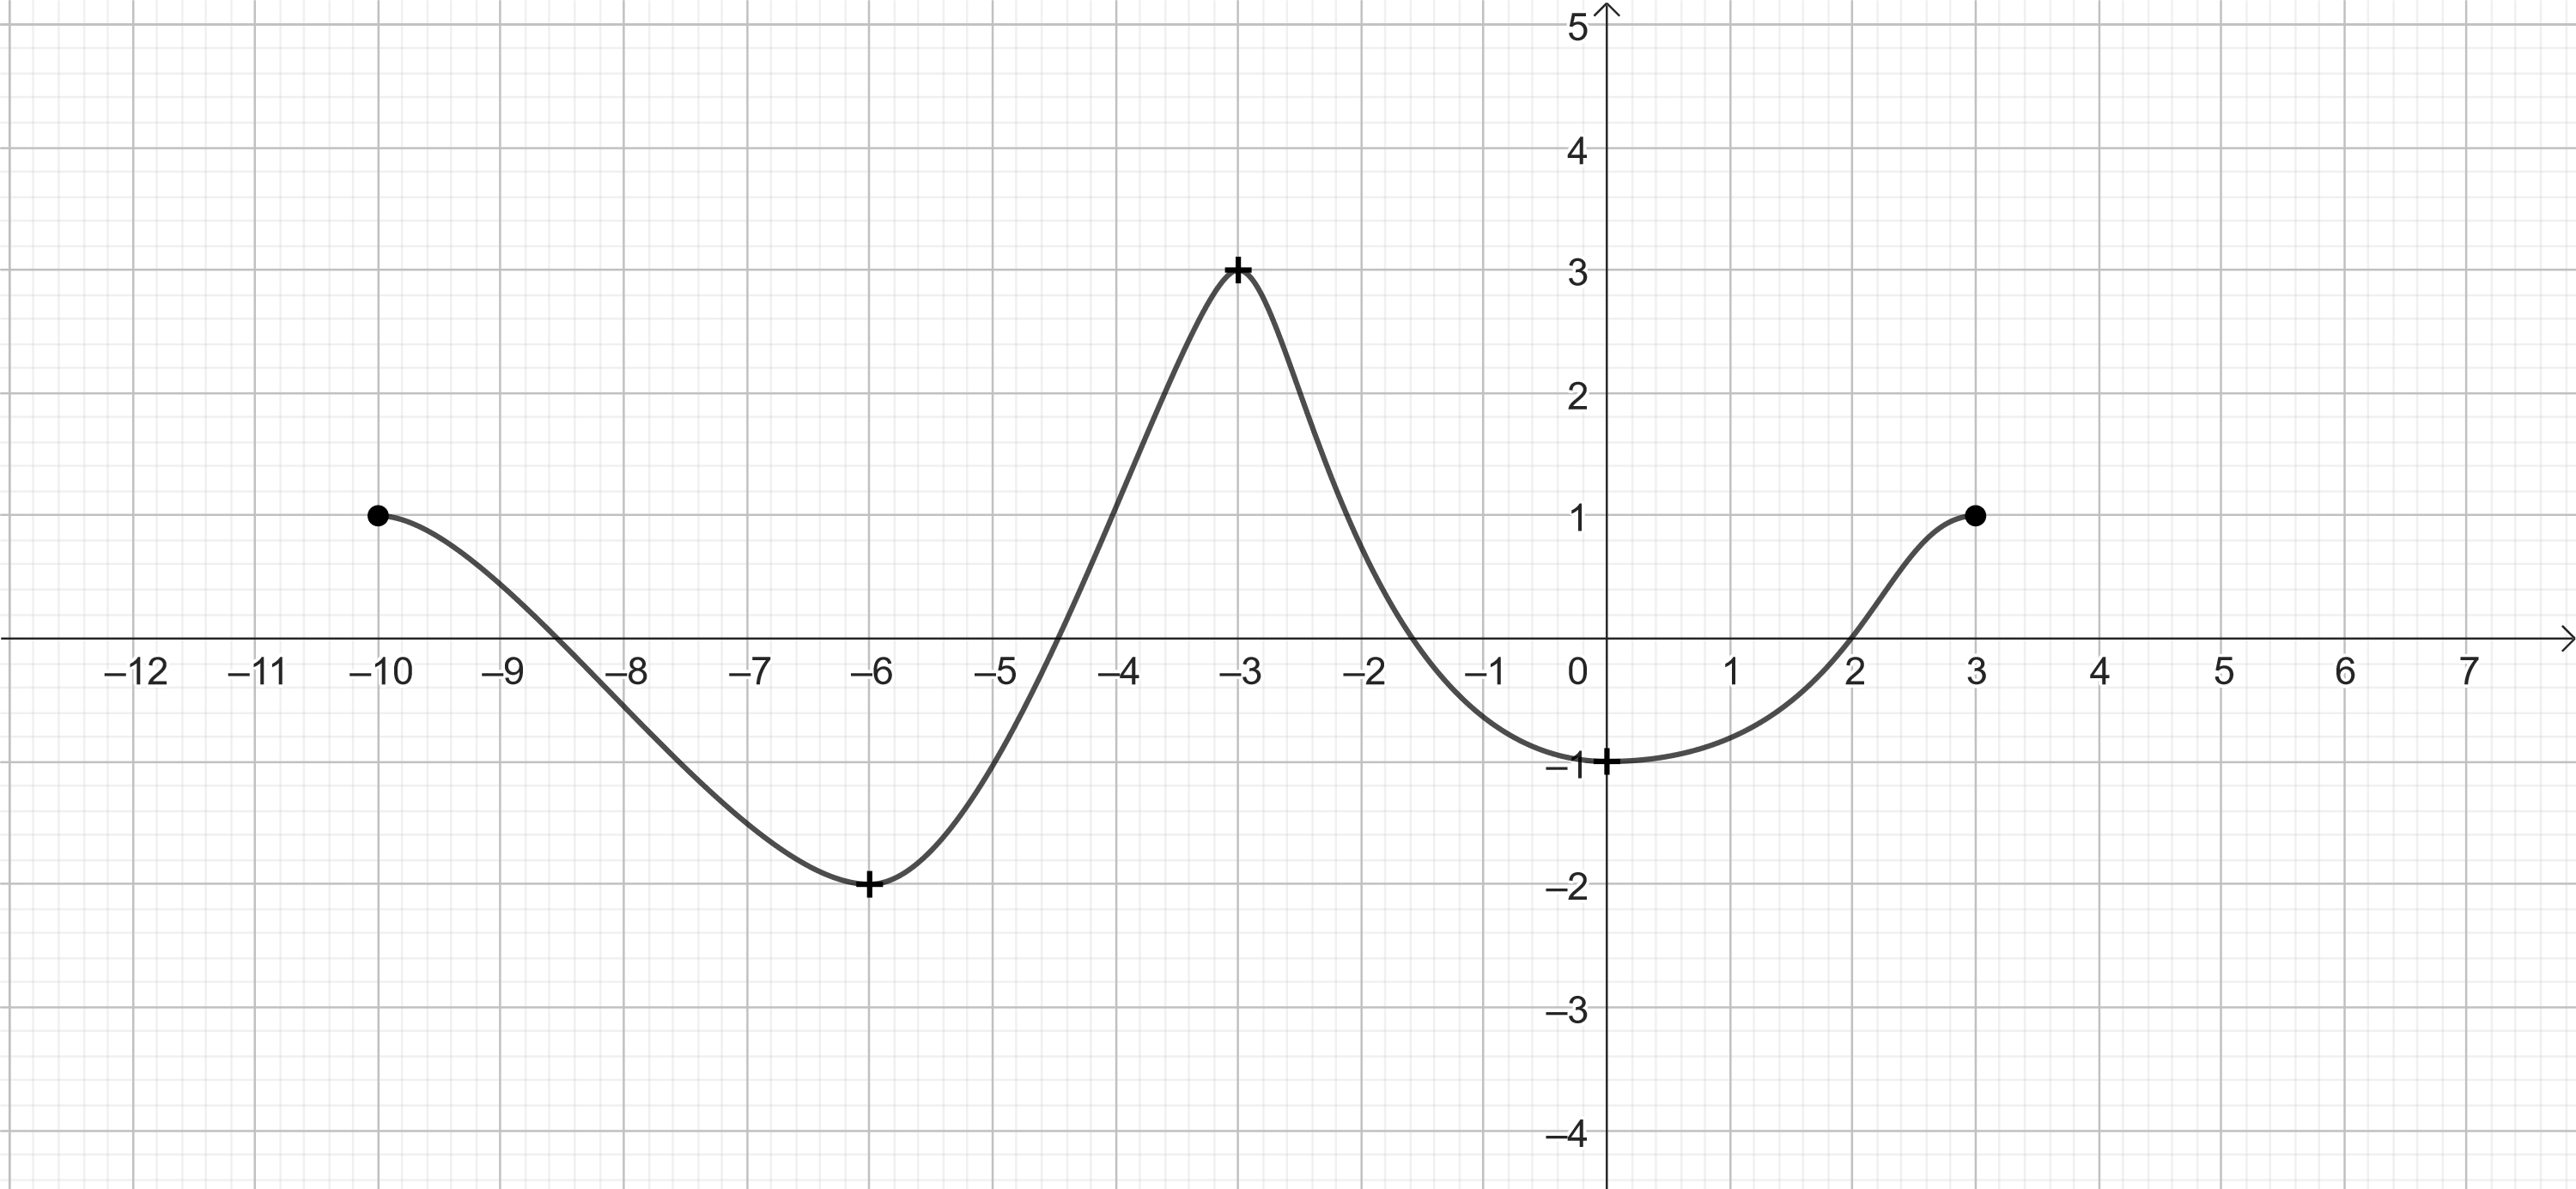
\includegraphics[width=0.9\textwidth]{Controle1.png}
\end{center}
\begin{parts}
\part Donner l'ensemble de définition de la fonction.
\part Compléter le tableau de variation de $f$.
\begin{center}
\begin{tikzpicture}
\tkzTabInit{$x$ / 0.5, Variations de $f$ / 2}{,,,};
\end{tikzpicture}
\end{center}
\part Quels sont le maximum et le minimum de $f$ ? 
\part En quelles valeurs $f$ atteint son maximum ? Et son minimum ?
\part Comparer $f(-6)$ et $f(1)$.
\end{parts}
\vspace*{1cm}
\titledquestion{Variations de fonctions : Episode 2, le retour de la géométrie}[4]
La comète de Halley, nommée en l'honneur de son découvreur Edmond Halley, est un corps céleste visible à l'oeil nu tous les $75$ ans environ.

On s'intéresse à la simulation de la trajectoire d'une comète proche de la Terre. L'unité utilisé dans cet exercice est l'unité astronomique. La Terre est assimilée à un point $T(3;2)$. À l'instant $t$, la comète est alors assimilée à un point $H(6-6t;2+4t)$. On admet que la trajectoire de la comète est alors donnée par une droite, que l'on nommera $(d)$.
\begin{center}
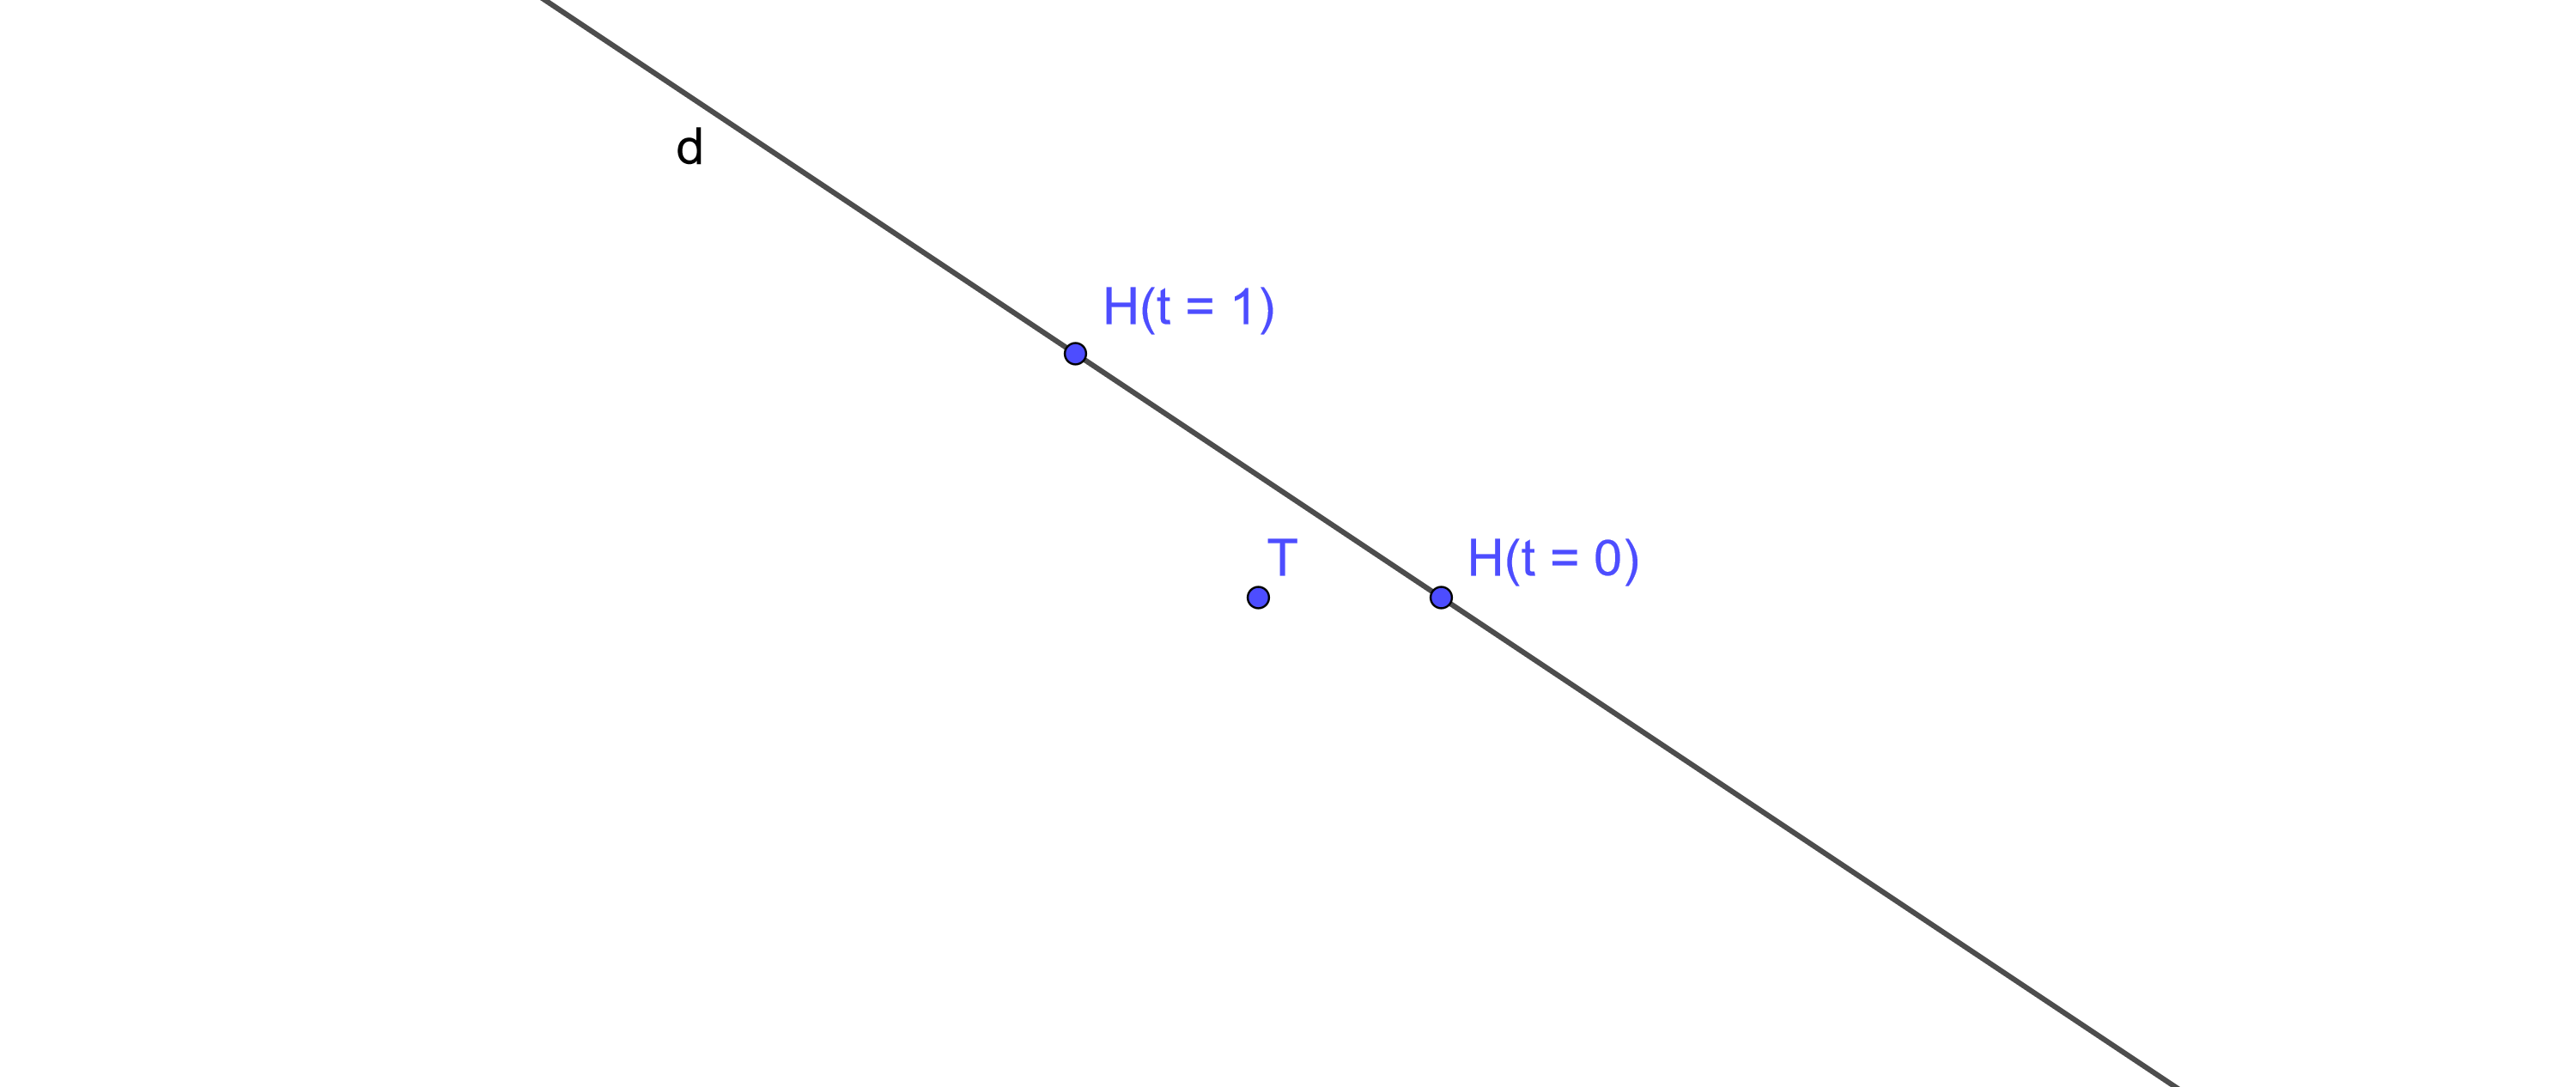
\includegraphics[width=0.9\textwidth]{Controle2.png}
\end{center}
\begin{parts}
\part Justifier que la distance $TH = 3$ quand $t = 0$.
\part Justifier que la distance $TH = 5$ quand $t = 1$.
\part On note $h(t)$ la distance $TH$ à chaque instant $t$. Démontrer que
\begin{equation*}
h(t) = \sqrt{52t^2 - 36t + 9}    
\end{equation*}
\part La courbe représentative de la fonction $h$, restreinte à l'intervalle $\left[0;2\right]$, est donnée ci-après.
\begin{center}
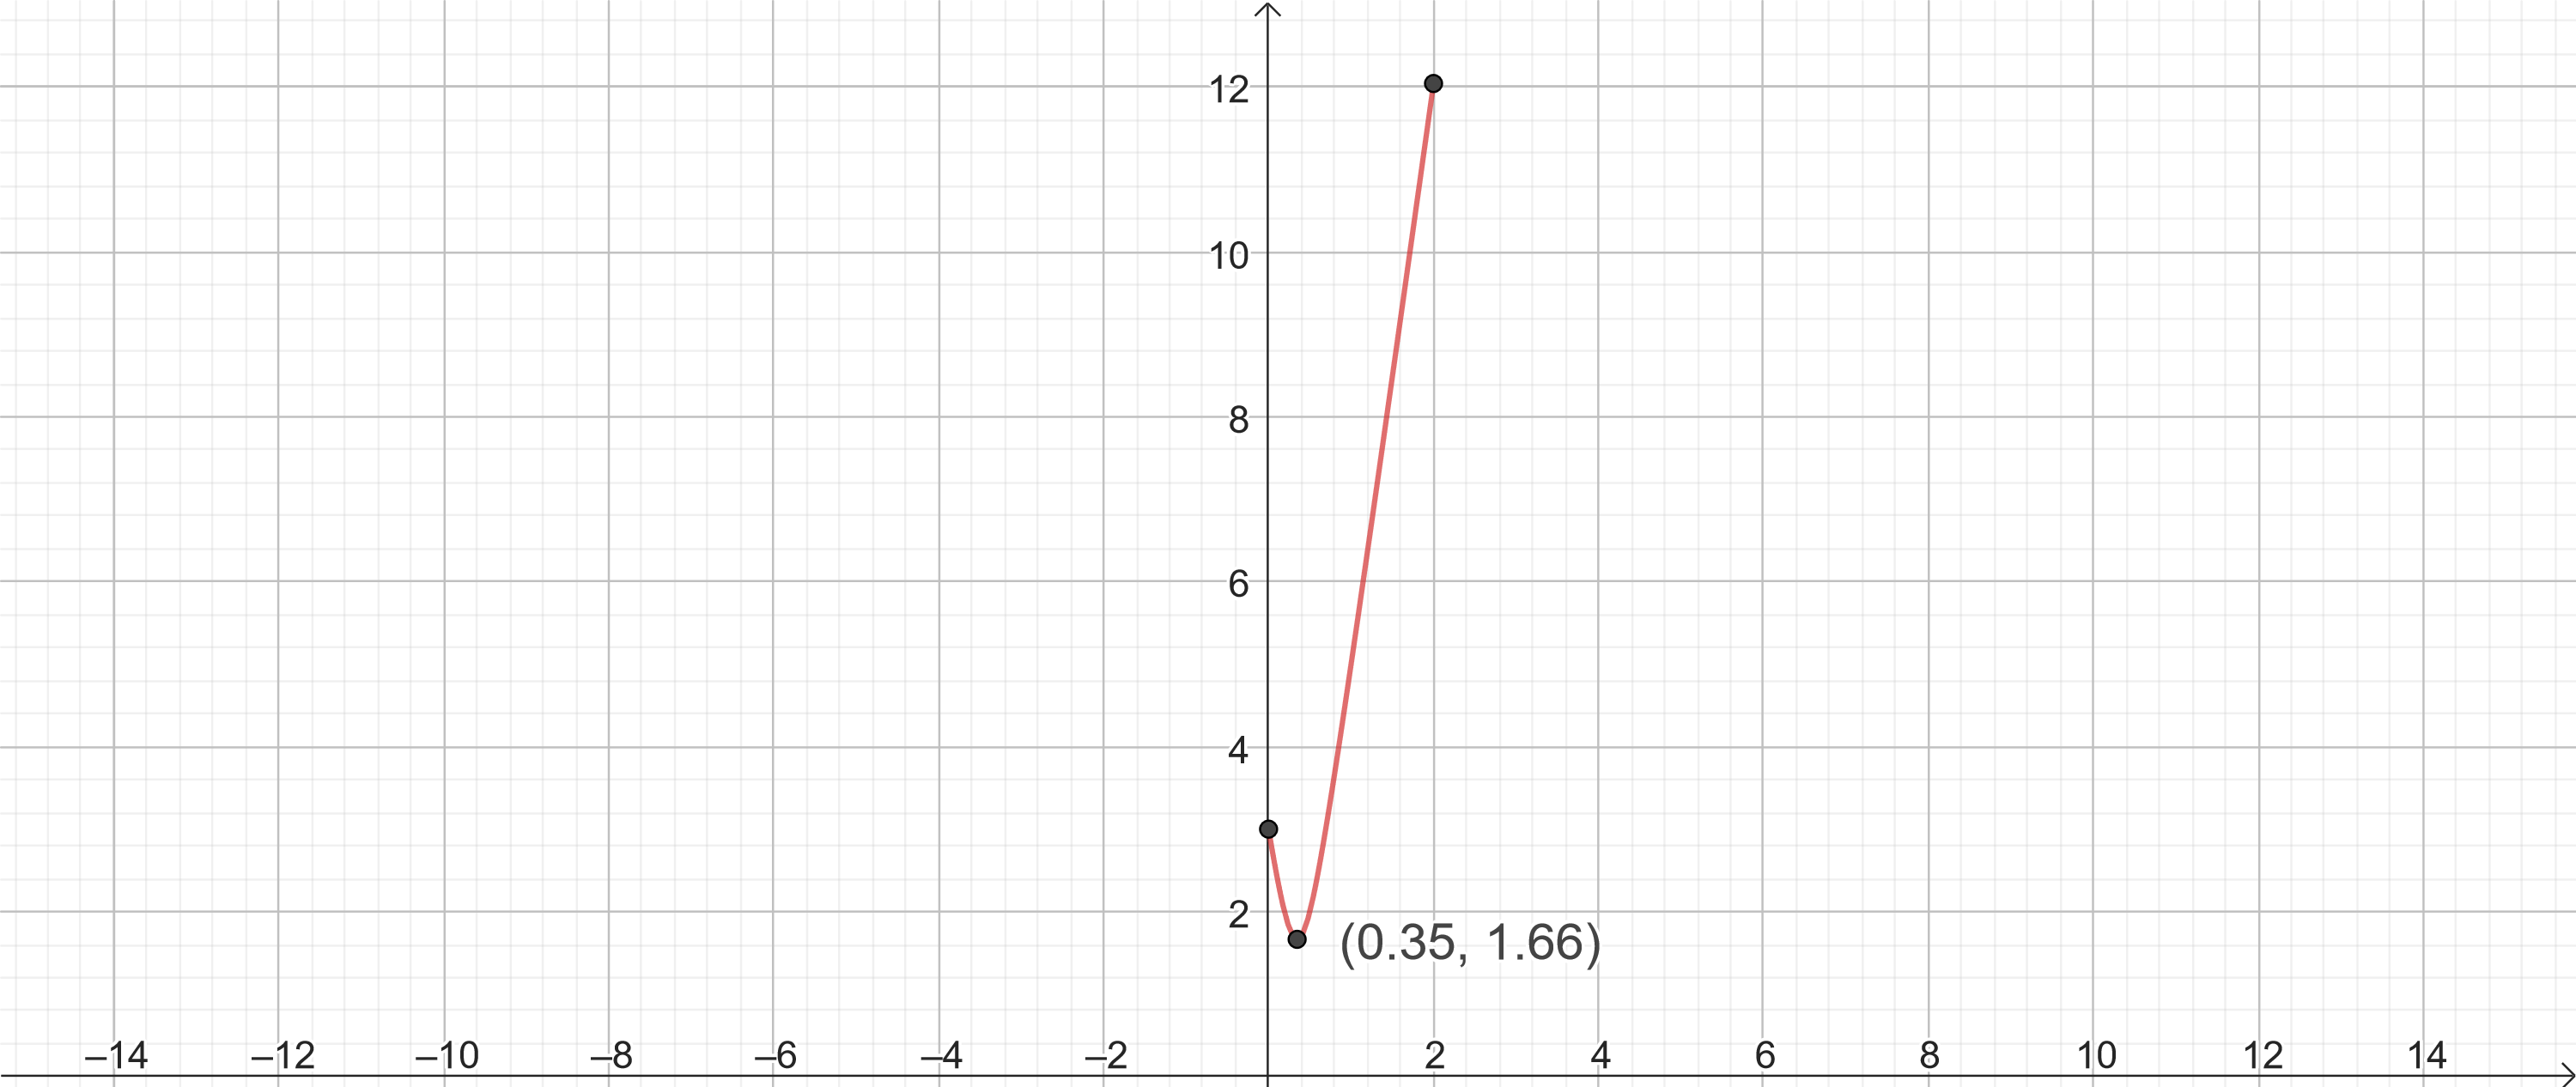
\includegraphics[width=0.9\textwidth]{Controle3.png}
\end{center}
À quel instant $t$ la comète est-elle la plus proche de la Terre ?
\end{parts}
\vspace*{1cm}
\titledquestion{Variations de fonctions : Episode 3, la fonction invisible}[4]
On teste un nouveau médicament sur un cobaye conscient. L'injection dure $60$ minutes, temps durant lequel la concentration du médicament dans le sang augmente, puis le médicament est progressivement éliminé de l'organisme, jusqu'à être absent au bout de $4$ heures. On note $c(t)$ la concentration du médicament dans le sang, en $\si{\milli\gram\per\liter}$, en fonction du temps $t \in \left[0;4\right]$, en heures.
\begin{parts}
\part Que vaut $c(0)$ ? Et $c(4)$ ?
\part On pose $c(0,5) = 500$. 
\part Compléter le tableau de variations suivant pour obtenir un tableau de variations possible pour $c$.
\begin{center}
\begin{tikzpicture}
\tkzTabInit{$t$ / 0.5, Variations de $c$ / 2}{,,};
\end{tikzpicture}
\end{center}
\part Dessiner une courbe représentative possible pour $c$, et telle que $c(0,5) \leq c(1,5)$.
\end{parts}
\vspace*{1cm}
\bonustitledquestion{Fonctions paires et impaires}[2]
Soit $f$ une fonction définie sur $\R$. On rappelle que $f$ est \emph{paire} si pour tout $x$, on a $f(-x)=f(x)$, et $f$ est \emph{impaire} si pour tout $x$, on a $f(-x)=-f(x)$. On suppose que $f$ est à la fois paire et impaire. Donner la valeur de $f(1)$, $f(2)$ et $f(3)$.
\end{questions}
\end{document}